\documentclass[10pt,twocolumn,letterpaper]{article}


\usepackage{cvpr}
\usepackage{times}
\usepackage{graphicx}
\usepackage{algorithm}
\usepackage{algorithmic}
\usepackage{url}
\usepackage{appendix}



\cvprfinalcopy % *** Uncomment this line for the final submission

\def\cvprPaperID{****} % *** Enter the CVPR Paper ID here
\def\httilde{\mbox{\tt\raisebox{-.5ex}{\symbol{126}}}}

% Pages are numbered in submission mode, and unnumbered in camera-ready
\ifcvprfinal\pagestyle{empty}\fi

\cvprfinalcopy
\ifcvprfinal\pagestyle{empty}\fi

\begin{document}

\title{An Implementation of the Active Contours without Edges Model and the Logic Framework for Active Contours on Multi-channel Images}

\author{Karim Ali and Sarah Nadi\\
\{karim, snadi\}@cs.uwaterloo.ca \\
CS870 - Fall 2010\\
David R. Cheriton School of Computer Science\\
University of Waterloo\\
}

\maketitle

\begin{abstract}
In this project, we provide an implementation for the Chan-Vese model for active contours without edges, and the Sandberg-Chan logic framework for active
contours on multi-channel images. The Chan-Vese model is a special case of the more general Mumford-Shah functional for segmentation and level sets. It
differs
from other active contour models in that it is not edge dependent, therefore it is more capable of detecting objects whose
boundaries may not be defined by a gradient (e.g. blurry images, noisy images). The Sandberg-Chan model builds on top of the Chan-Vese model by allowing the
contour to evolve simultaneously on multiple channels. It also offers a set of logic operations that can be applied to those channels (union, intersection,
complement, and their combinations). We evaluate our implementation based on several criteria, such as: independence of initial curve position, successful
detection of holes, performance with blurred and noisy images, and response to scaling parameters.
\end{abstract}


\section{Introduction}
Image segmentation or boundary detection is a very important problem in the area of Image Processing, and has received a lot of attention in the past. The
classical Active Contour model (or Snakes) proposed by Kass et al.~\cite{kass1988snakes} was the first model to use the idea of energy minimization to attract
a contour to the edges of the objects in an image. The Snakes model was very successful and variations of it were highly adopted later on
(E.g.~\cite{caselles1997geodesic}. Most of these models use the level set formulation for propagating fronts to evolve the curve. However, these models highly
depend on motion defined by the gradient of the image which leads to poor performance in smoothed edges. To overcome these limitations, Chan
and Vese~\cite{chan2001active} propose an active contour model that does not depend on the edges (i.e the gradient) for propagating the curve to detect the
boundary of the object. Instead, they use a region-based approach based on the Mumford-Shah model \cite{mumford1989optimal} to divide the image
into two regions: one inside the propagating curve, and one outside. The curve is at the boundary of the object if there is no difference in intensities inside
the curve as well as outside the curve.

The Active Contours without Edges model proposed by Chan and Vese (referred to as Chan-Vese model throughout the rest of this paper) is very successful in
detecting objects even in noisy or blurry images. It can also detect holes in objects which is usually a limitation in previous models. As an extension to
this work, Sandberg and Chan~\cite{sandberg2005logic} propose a logic framework (referred to as the Sandberg-Chan model throughout the rest of this
paper) that  performs logic operations on multiple images according to the curve propagation proposed in the Chan-Vese model. To achieve that, previous models
usually had two steps. They would either first segment the object in each channel separately then combine the segmented objects according to the logic operation
through bitwise operations~\cite{sapiro1997color, zhu2002region} or they would apply logic operations to the different images then segment the resulting
image. The first approach is
very costly, and the second approach requires a lot of prior knowledge about the intensities of each image. To overcome these drawbacks, the Sandberg-Chan
model is based on the idea of fitting a single contour to the object on all channels according to the logic operator, and based on regions.

\begin{figure}[t]
\centering
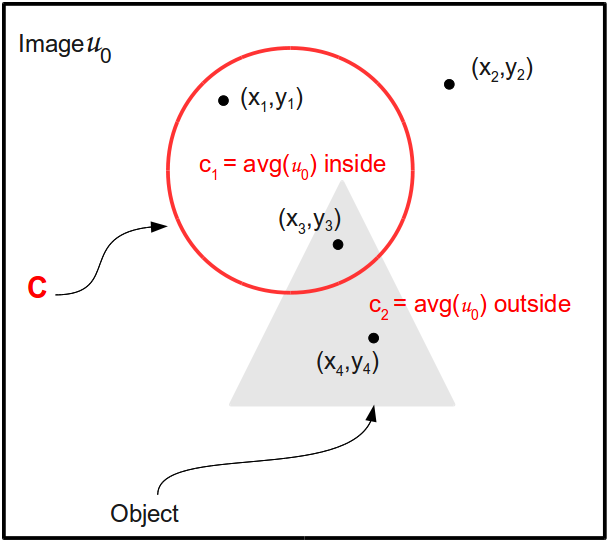
\includegraphics[width=6cm]{explaining.png}
\caption{Region Based Model}
\label{fig:region}
\end{figure}

In this paper, we report on our findings after implementing each of these models. We implement both models in Matlab, and experiment with several images.
We explain the details of our implementation as well as our results. The rest of this paper is organized as follows:
Section~\ref{sec:bg} provides brief background about each of the two models implemented in this paper. Section~\ref{sec:implementation} then explains our
implementation. In this section, we explain how we implemented the models and any variations from the original papers. Section~\ref{sec:results} explains our
evaluation criteria, and
presents the results we obtained. Section~\ref{sec:difficulties} discusses some of the difficulties we faced during implementation. Section~\ref{sec:concl}
concludes this paper by summarizing our findings.

\section{Background}
\label{sec:bg}


\subsection{Chan-Vese Model}
\label{sec:chan-vese}

The Chan-Vese model~\cite{chan2001active} is a region based model for detecting objects in an image. It is based on a restriction of the Mumford-Shah model
which divides an image into
regions and represents each region by a piecewise constant (also called the minimal partition problem). Figure~\ref{fig:region} shows this region based model.
The figure shows an image $u_{0}$ which has a gray triangular object in it. The red curve, $C$, is the initial contour used to detect this object. The
main idea behind the model is that the curve divides the image into two regions: that inside the curve and that outside. Each region is represented by a
constant, $c$, which is the average intensity of the image values in each region. In order for the curve to fit the object, there must be minimal variation of
the
intensities inside the curve as well as outside. In other words, this turns into a minimization problem of the difference of intensities inside (fitting term
one, $F_{1}$) plus those
outside (fitting term two, $F_{2}$). For example, in Figure~\ref{fig:region}, the point $(x_{1},y_{1})$ will have to be outside the curve in order to minimize
the difference
between the points inside
the curve. Similarly, the point $(x_{4}, y_{4})$ will have to be inside the curve. Figure~\ref{fig:fitting} shows all the possibilities of the curve's fitting
according to its position with respect to the object.

More formally, the Euler-Lagrange equation (as derived in the original paper) representing the time motion of the curve $C$ is shown in
Equation~\ref{eqn:cvpde}.

\begin{equation}
\label{eqn:cvpde}
\frac{\partial{\phi}}{\partial{t}} = \delta_{\varepsilon}(\phi)[\mu\; \mathrm{div}(\frac{\bigtriangledown \phi}{|\bigtriangledown \phi|}) - \nu -
\lambda_{1}(u_{0} - c_{1})^2 +\lambda_{2}(u_{0} - c_{2})^2] 
\end{equation}

\begin{figure}[t!]
\centering
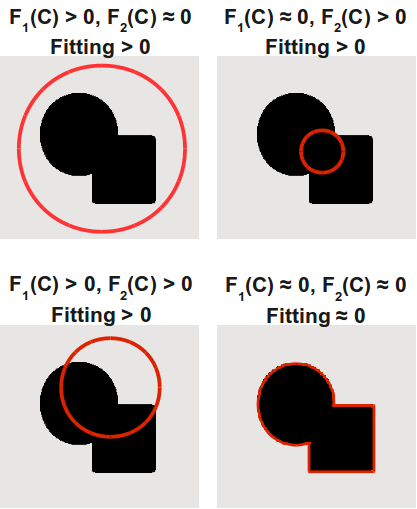
\includegraphics[width=6cm]{fitting.png}
\caption{Chan-Vese Curve Fitting}
\label{fig:fitting}
\end{figure}

The parameter $\mu$ is a scaling parameter for the length of the curve represented in terms of curvature. The smaller $\mu$ is, the more the length of the curve
can increase without penalizing the minimization. This allows the model to detect smaller objects and holes. The larger $\mu$ is, the less freedom there is for
the curve to increase in length, and thus, it will only be able to detect larger objects. The parameter $\nu$ is also a scaling term for the area of the curve.
However, the authors do not use the area term in the Euler-Lagrange derivation, and always set $\nu$ to 0. It seems that $\mu$ is sufficient to scale the curve
according to the objects that need to be detected. Finally, $\lambda_{1}$ and $\lambda_{2}$ are weighting parameters for the forces inside the curve and
outside the curve respectively. Since we want to give both forces equal weight, the authors set $\lambda_{1} = \lambda_{2} = 1$ in all their experiments.


\begin{figure*}[t]
\centering
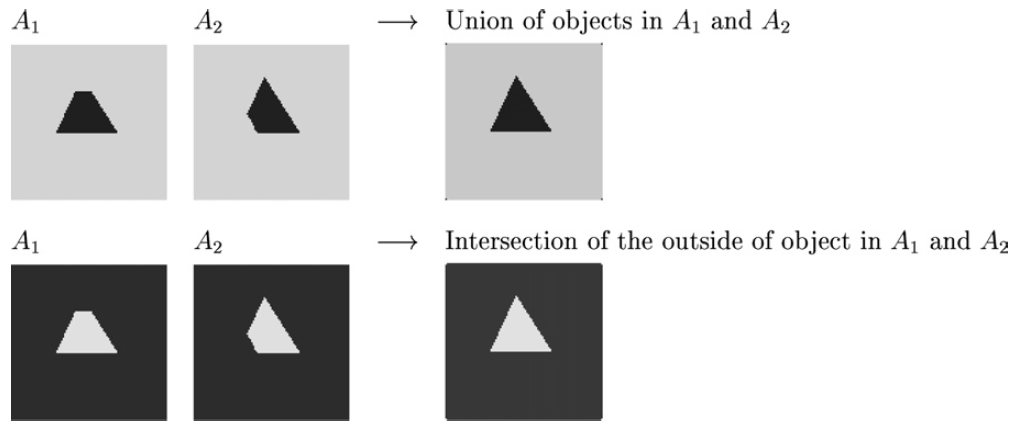
\includegraphics[width=0.7\textwidth]{logicop.png}
\caption{Region Based View Union}
\label{fig:logic-op}
\end{figure*}


\subsection{Sandberg-Chan Model}
\label{sec:sandberg-chan}

The main goal of the Sandberg-Chan model~\cite{sandberg2005logic} is to perform logic operations on a combination of different images accurately and
efficiently. For example, finding the union of two images where different parts of the object are occluded in each image so that a complete object can be
obtained. This example will be shown later in Figure~\ref{fig:family}. In order to do that, they use the Chan-Vese model to detect objects, and simultaneously
include the logic operations in the minimization problem.
Since they are using the Chan-Vese model, the problem must be viewed in terms of regions as well. Accordingly, they define the two main logic operations
(union and intersection) in terms of regions where the union of two images is the union of the inside of the curve with respect to the images plus the
intersection of the outside of the curve with respect to the images. For example, Figure~\ref{fig:logic-op}~\cite{sandberg2005logic} shows that the
union of $A_{1}$ and $A_{2}$ (in terms of its shape) can be obtained by taking the union of the insides of the object or the intersection of the outsides.
Similarly, the intersection of two images would be the intersection of the insides plus the union of the outsides. Thus, in order to obtain accurate results
irrespective of the object's intensity outside versus inside, we should consider \textit{both} the logic operation required for the region inside the object
as well as that outside.



More formally, the authors define two logic variables $z_{i}^{in}$ and $z_{i}^{out}$ to denote whether a point $(x,y)$ should be in the moving curve $C$ or not
with respect to image $i$. Since we are trying to minimize the fitting of the curve, they use $0$ to denote $true$ and $1$ to denote $false$ (the reverse of the
usual
convention). Following the Chan-Vese model, they represent each of the regions inside and outside the curve by a constant $c$. In this paper, they represent
$c_{in}$ as $c_{+}$ and $c_{out}$ as $c_{-}$. Equations~\ref{eqn:zin} and~\ref{eqn:zout} show how to calculate $z_{in}$ and $z_{out}$ respectively in terms of
the Chan-Vese model. We note here that in the original paper there was a typo in these equations where they divide by the maximum intensity of each image
instead of the maximum intensity squared. However, in order to have $z_{in}$ and $z_{out}$ have values from 0 to 1 that represent logic values, we need to
divide by the maximum intensity squared. The equations shown below have been corrected for that.


\begin{equation}
\label{eqn:zin}
z_{i}^{in}(u_{0}^{i},x,y,C) = \frac{|u_{0}^{i} - c_{+}^i|^2}{(max_{(x,y) \in u_{0}^{i}} u_{0}^i)^2}
\end{equation}

\begin{equation}
\label{eqn:zout}
z_{i}^{out}(u_{0}^{i},x,y,C) = \frac{|u_{0}^{i} - c_{-}^i|^2}{(max_{(x,y) \in u_{0}^{i}} u_{0}^i)^2}
\end{equation}

In order to perform logic operations on $z_{in}$ and $z_{out}$, the authors introduce interpolation functions that mimic the behavior of the regular truth
table, but for continuous values between 0 and 1. The union and intersection functions for two variables are shown in Equations~\ref{eqn:funion}
and~\ref{eqn:finters} respectively. These equations can be simply extended to any number of variables.

\begin{equation}
\label{eqn:funion}
f_{\cup} = (z_{1} . z_{2})^{1/2}
\end{equation}

\begin{equation}
\label{eqn:finters}
f_{\cap} = 1 - ((1 - z_{1}) .(1-  z_{2}))^{1/2}
\end{equation}

Based on these functions, the Euler-Lagrange equation for any logic operation is shown in Equation~\ref{eqn:svpde}. According to the desired logic operation,
$f_{in}$ and $f_{out}$ will be specified. For example, if we are doing the union of the images, then we will need to perform a union operation on
the insides. Thus, $f_{in}$ will be replaced by Equation~\ref{eqn:funion}. Similarly, we will need to do the intersection of the outsides so $f_{out}$ will be
replaced by Equation~\ref{eqn:finters}.

\begin{table*}[h!t!]
\centering
\resizebox{\textwidth }{!}{
\begin{tabular}{ c | c |c}
\textbf{Criteria} & \textbf{Goal} & \textbf{Applies to Model}\\
\hline\hline
Detecting Boundaries & Ability to correctly detect object boundaries of simple objects& Both Models\\
\hline
Curve Position & Ability to correctly detect object boundaries irrespective of the initial curve position & Both Models\\
\hline
Detecting Holes & Ability to detect holes in objects, and not simply stop on outside boundary & Both Models\\
\hline
Blurred Images & Ability to correctly (as much as possible) detect object boundaries in blurred images & Both Models\\
\hline
Noisy Images & Ability to correctly (as much as possible) detect object boundaries in noisy images & Both Models\\
\hline
Union Operator & Ability to correctly obtain the union of two or more images & Sandberg-Chan\\
\hline
Intersection Operator & Ability to correctly obtain the intersection of two or more images & Sandberg-Chan\\
\hline
Complement & Ability to correctly obtain the union or intersection of two or more images containing complements & Sandberg-Chan\\
\hline
Parameter Settings & Ability to respond correctly to the different parameter settings & Both Models\\
\end{tabular}
}
\centering
\caption{Evaluation Criteria}
\label{tab:criteria}
\end{table*}



\begin{equation}
\label{eqn:svpde}
\frac{\partial{\phi}}{\partial{t}} = \delta(\phi)[\mu\bigtriangledown(\frac{\bigtriangledown \phi}{|\bigtriangledown \phi|})  - \lambda(f_{in}(z_{1}^{in}, ...,
z_{n}^{in}) - f_{out}(z_{1}^{out}, ..., z_{n}^{out})
\end{equation}


\section{Implementation}
\label{sec:implementation}

During implementation, we tried to stick to the authors' formulas and guidelines as much as possible. In this section we explain what methods we use to
numerically solve the PDEs. For the chan-vese model, we use the PDE given in Equation 9 in the original paper~\cite{chan2001active} which is shown in
Equation~\ref{eqn:cvpde}.  We, first, tried to implement the dirac delta function, $\delta_{\varepsilon}\phi$, as defined in the paper. However, it resulted in
worse segmentations. Accordingly, we chose to use $|\bigtriangledown\phi|$ instead of the dirac delta function as this
was indicated as a valid alternative by the authors. To calculate $c_{1}$ and $c_{2}$, we simply calculated the mean of the values inside $\phi$ (specifically
where $\phi > 0$) and the mean of the values outside $\phi$ (specifically where $\phi < 0$) respectively. To actually solve the PDE, we chose to use an explicit
time stepping scheme for the finite difference discretization. That is, in each time step $\phi^{n+1} = \phi^n + \triangle t*\phi_t$. This was simpler to
implement, and although $\triangle t$ must be chosen carefully to satisfy the stability condition ($\triangle t <= (1/imageSize)^2$), we did not suffer from
performance problems due to this restriction.

For the Sandberg-Chan model, we used the PDE given in original paper as well, and shown in Equation~\ref{eqn:svpde}. Again, we used $|\bigtriangledown\phi|$
instead of the dirac delta function. We calculated $z_{in}$ and $z_{out}$ according to Equations~\ref{eqn:zin} and~\ref{eqn:zout} shown above which have been
corrected for
the typo in the original paper. For all other equations and calculations necessary in the model, we closely followed the original paper in our implementation.
We also used an explicit time stepping scheme in this model. 

We use the same stopping condition for both model. That is, to check if we have reached the stationary solution, we check if more points have been added inside
the contour or not. More formally, we check if $(\phi^{n+1} > 0) == (\phi_{n} > 0)$. If the contour did not move, then new points will be added to its inside,
and this condition will be satisfied.


\section{Experimental Results}
\label{sec:results}

In order to make sure we correctly implemented the models, we had several evaluation criteria. Table~\ref{tab:criteria} summarizes these criteria, and explains
the goals of each. Some of these criteria apply for both models, while other apply to one or the other. For the rest of this section, we proceed by presenting
our experimental results for both models. For each model, we proceed in the order of these criteria starting with the simplest
cases, and incrementally challenging the model. Unless otherwise stated, all the segmentation was performed on a gray scale version of the original image. All
the images in the Chan-Vese model were run on an Intel Core 2 Duo processor with 2.00 GHz and a 2GB RAM and all the images in the Sandberg-Chan
model were run on a Intel Centrino Duo 2.0 processor and a 1GB RAM computer. As shown in the results,
we tried different image sizes to ensure that our solution converges.



\subsection{Chan-Vese Model Results}

We present the results from the Chan-Vese model in this section, and show which criteria were met and which were not. Unless otherwise specified, we set
$\lambda_{1} = \lambda_{2} = 1$.

\begin{figure}[t]
\centering
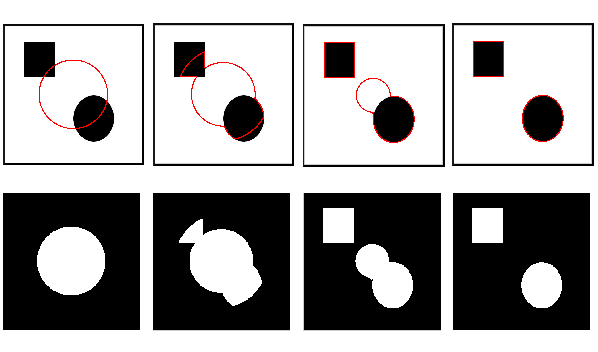
\includegraphics[width=0.5\textwidth]{cv_eg1.png}
\caption{Successful detection of object boundaries. Top: the evolving curve (in red) over time where the first image shows the initial contour.
Bottom: evolving segmentation over time until the objects are detected. Size = 300 x 300, $\phi_{0}(x,y) = - \sqrt{(x - 150)^2 + (y - 150)^2} + 75$, $\mu =
0.01$, no reinitialization, cpu = 2.9s, iterations = 7.}
\label{fig:cv_eg1}
\end{figure}

\begin{figure*}[t]
\centering
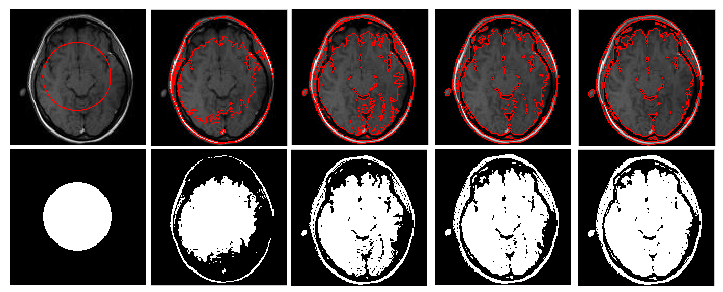
\includegraphics[width=12cm]{cv_eg2.png}
\caption{Successful detection of object boundaries. Top: the evolving curve (in red) over time where the first image shows the initial contour.
Bottom: evolving segmentation over time until the object is detected. Size = 131 x 131, $\phi_{0}(x,y) = - \sqrt{(x - 65.6)^2 + (y - 65.5)^2} + 32.8$, $\mu =
0.01$, no reinitialization, cpu = 1.95 s, iterations = 7.}
\label{fig:cv_eg2}
\end{figure*}

\subsubsection*{Successful Detection of Boundaries}

Figure~\ref{fig:cv_eg1} shows that the implemented model can successfully detect object boundaries in a simple image. In this case, the evolving curve was
successfully able to detect the boundaries of both objects. Figure~\ref{fig:cv_eg2} shows a slightly more complicated example where the evolving contour
successfully detects the contour of the brain. Note that there is a tiny area near the center to the left of the brain that was also successfully detected. To
ensure
that open boundaries (e.g. lines) can also be detected, we used an image with several shapes shown in Figure~\ref{fig:cv_eg8}.

\begin{figure*}[t]
\centering
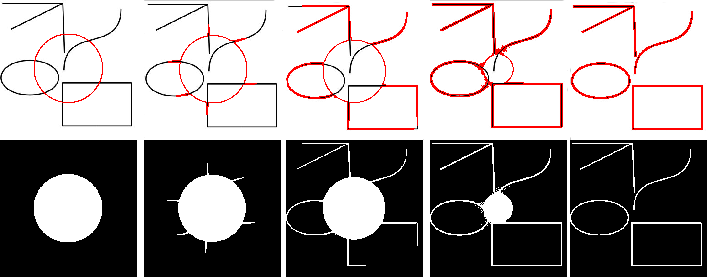
\includegraphics[width=12cm]{cv_eg8.png}
\caption{Successful detection of object with open boundaries. Top: the evolving curve (in red) over time where the first image shows the initial contour.
Bottom: evolving segmentation over time until all objects are detected. Size = 300 x 300, $\phi_{0}(x,y) = - \sqrt{(x - 150)^2 + (y - 150)^2} + 75$, $\mu =
0.01$, no reinitialization, cpu = 5.19 s, iterations = 11.}
\label{fig:cv_eg8}
\end{figure*}


\begin{figure*}[t!]
\centering
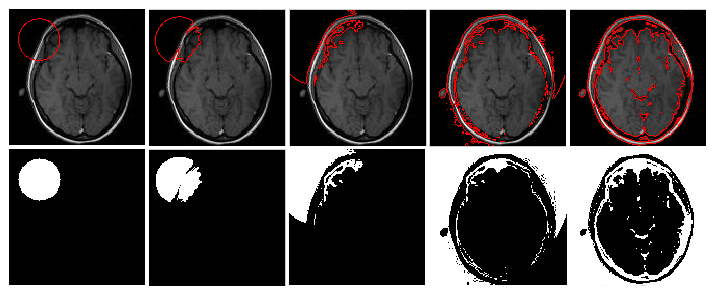
\includegraphics[width=12cm]{cv_eg3.png}
\caption{Initial curve position partially overlapping object. Top: the evolving curve (in red) over time where the first image shows the initial contour.
Bottom: evolving segmentation over time until the object is detected. Size = 131 x 131, $\phi_{0}(x,y) = - \sqrt{(x - 30)^2 + (y - 30)^2} + 20$, $\mu =
0.01$, no reinitialization, cpu = 2.26 s, iterations = 9.}
\label{fig:cv_eg3}
\end{figure*}

\begin{figure*}[t!]
\centering
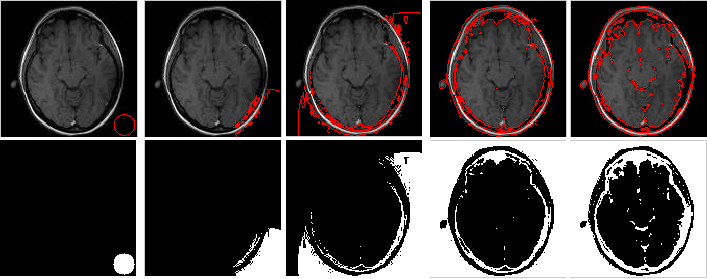
\includegraphics[width=12cm]{cv_eg4.png}
\caption{Initial curve position not overlapping any area of the object. Top: the evolving curve (in red) over time where the first image shows the initial
contour. Bottom: evolving segmentation over time until the object is detected. Size = 300 x 300, $\phi_{0}(x,y) = - \sqrt{(x - 120)^2 + (y - 120)^2} + 10$,
$\mu =0.01$, no reinitialization, cpu = 2.01 s, iterations = 9.}
\label{fig:cv_eg4}
\end{figure*}

\subsubsection*{Independence of Initial Curve Position}


To ensure that the initial position of the curve does not affect the final segmentation, we tested two other positions for the initial curve for the same
brain image
used in Figure~\ref{fig:cv_eg2}. In Figure~\ref{fig:cv_eg2}, the initial contour was completely overlapping the object. Accordingly, we tried two other
positions. The first one is shown in Figure~\ref{fig:cv_eg3} where the initial contour only partially overlaps with the object. The second one is shown in
Figure~\ref{fig:cv_eg4} where the initial contour does not overlap the object in any part. Visually, the obtained segmentation was the same with a slightly
higher number of iterations and CPU time. In all three cases, the brain was correctly segmented. We compared the area segmented as the brain in each case to
make sure the same segmentation was obtained, and in each case, we got the same area of 0.5268. Note, however, that when part of the curve lies outside the
object, the definition of inside and outside changes since the curve becomes an open curve at one point. This should not make a difference as long as the
contour lies correctly at the boundaries of the object. 

\begin{figure*}[t]
\centering
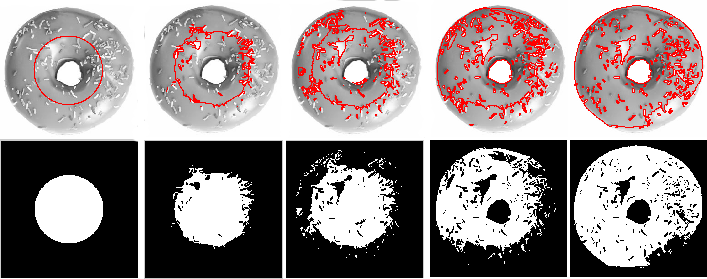
\includegraphics[width=12cm]{cv_eg5.png}
\caption{Successful detection of holes.  Top: the evolving curve (in red) over time where the first image shows the initial
contour. Bottom: evolving segmentation over time until the object is detected. Size = 131 x 131, $\phi_{0}(x,y) = - \sqrt{(x - 65.5)^2 + (y - 65.5)^2} + 32.8$,
$\mu =0.01$, no reinitialization, cpu = 8.12 s, iterations = 12.}
\label{fig:cv_eg5}
\end{figure*}

\begin{figure*}[t!h!]
\centering
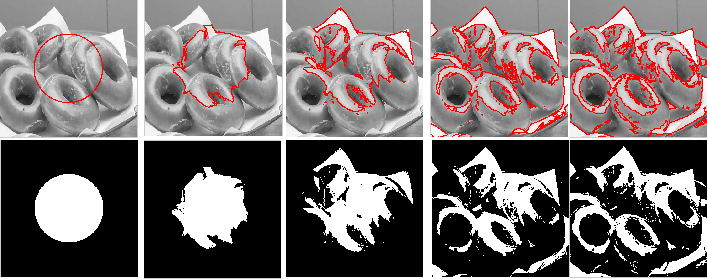
\includegraphics[width=12cm]{cv_eg6.png}
\caption{Successful detection of multiple holes.  Top: the evolving curve (in red) over time where the first image shows the initial
contour. Bottom: evolving segmentation over time until the object is detected. Size = 300 x 300, $\phi_{0}(x,y) = - \sqrt{(x - 150)^2 + (y - 150)^2} + 75$,
$\mu =0.01$, no reinitialization, cpu = 15.07 s, iterations =  23.}
\label{fig:cv_eg6}
\end{figure*}

\begin{figure}[t]
\centering
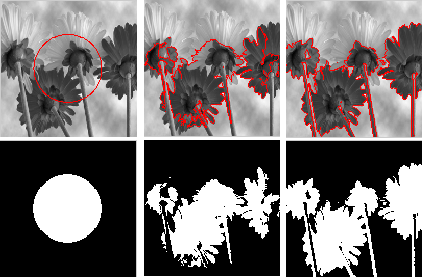
\includegraphics[width=0.5\textwidth]{cv_eg7.png}
\caption{Inability to detect low intensities that do not have much variation from their background.  Top: the evolving curve (in red) over time where the
first
image shows the initial
contour. Bottom: evolving segmentation over time until the object is detected. Size = 300 x 300, $\phi_{0}(x,y) = - \sqrt{(x - 150)^2 + (y - 150)^2} + 75$,
$\mu =0.01$, no reinitialization, cpu = 1.35 s, iterations = 6.}
\label{fig:cv_eg7}
\end{figure}



\subsubsection*{Successful Detection of Holes}

In order to make sure the contour does not simply stop at the outside boundary of an object and ignore any details inside such as holes, we tried two donut
images. Figure~\ref{fig:cv_eg5} shows how the curve is able to detect the hole in the donut. Additionally, it is able to detect the various sprinkles on it.
We note that the bottom right boundary is not very exact, and this is because the lighting effect in the image makes the intensity of this area very close to
that of the background This is a known drawback of the Chan-Vese model since it only divides the image into two regions, and requires a big variation in
intensities for the curve to change. Figure~\ref{fig:cv_eg6} shows that multiple holes in an image can also be successfully detected. Another example showing
the inability to detect objects with intensities close to that of the background is shown in Figure~\ref{fig:cv_eg7} where the flower parts with very low
intensities are not detected. We will show that we can overcome this limitation with the Sandberg-Chan model for this particular example.


\subsubsection*{Reasonable Performance with Blurred Images}


Figure~\ref{fig:cv_eg9} shows how the contour behaves in a blurry image. The photographer was successfully detected. Additionally, other objects in the image
such as the tripod were found. However, objects with a very light intensity were again not detected.

\begin{figure*}[t!]
\centering
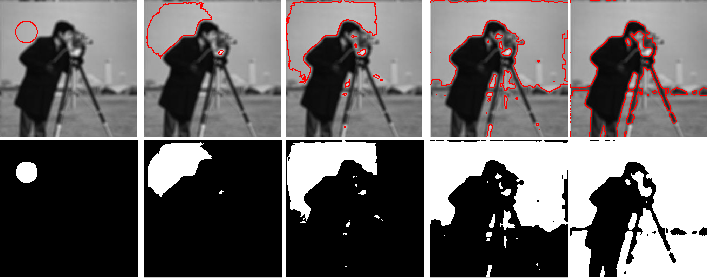
\includegraphics[width=12cm]{cv_eg9.png}
\caption{Ability to detect contours in blurry images.  Top: the evolving curve (in red) over time where the first
image shows the initial
contour. Bottom: evolving segmentation over time until the object is detected. Size = 255 x 255, $\phi_{0}(x,y) = - \sqrt{(x - 127.5)^2 + (y - 127.5)^2} +
63.75$, $\mu =0.01$, no reinitialization, cpu = 5.41 s, iterations = 15.}
\label{fig:cv_eg9}
\end{figure*}

\subsubsection*{Reasonable Performance with Noisy Images}


Figure~\ref{fig:cv_eg10} shows how two objects in a noisy image were successfully detected. In this image, we added a Gaussian noise with mean = 0 and
variation = 0.01
variance using Matlab's built-in noise function. The image shows that although some of the noise was detected in intermediate iterations, the contour continued
to evolve until it was only surrounding the desired objects. Unfortunately, the effect of noise was not completely ignored in all cases. For example,
Figure~\ref{fig:cv_eg11} shows that for the same image, but with \textit{Salt \& pepper} noise, the noise was detected as objects. This should not have been the
case
since we used a large value $\mu = 5$ for the length scaling parameter. However, varying $\mu$ does not have the intended effect as explained
in the next paragraph. 


\begin{figure*}[t]
\centering
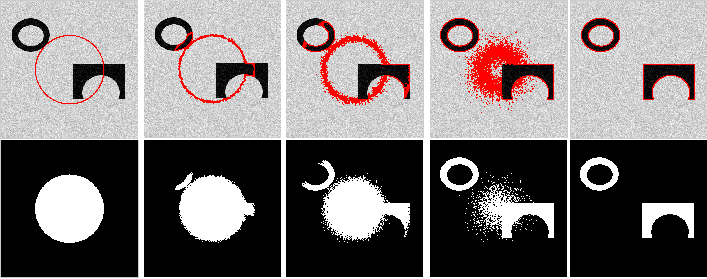
\includegraphics[width=12cm]{cv_eg10.png}
\caption{Ability to detect contours in an image with Gaussian noise.  Top: the evolving curve (in red) over time where the first
image shows the initial
contour. Bottom: evolving segmentation over time until the object is detected. Size = 300 x 300, $\phi_{0}(x,y) = - \sqrt{(x - 150)^2 + (y - 150)^2} +
75$, $\mu =0.01$, no reinitialization, cpu = 4.4 s, iterations = 7.}
\label{fig:cv_eg10}
\end{figure*}

\begin{figure*}[t!]
\centering
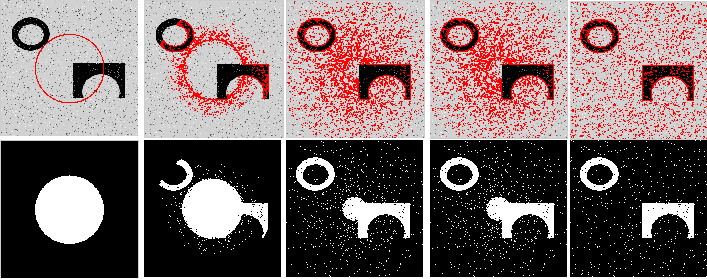
\includegraphics[width=12cm]{cv_eg11.png}
\caption{Figure~\ref{fig:cv_eg10}, but with \textit{Salt \& pepper} noise. Noise was still detected despite increasing $\mu$.  Top: the evolving
curve
(in red) over time where the first
image shows the initial
contour. Bottom: evolving segmentation over time until the object is detected. Size = 300 x 300, $\phi_{0}(x,y) = - \sqrt{(x - 150)^2 + (y - 150)^2} +
75$, $\mu = 5$, no reinitialization, cpu = 12.27 s, iterations = 7.}
\label{fig:cv_eg11}
\end{figure*}

\subsubsection*{Successful Response to Parameter Settings}

There are mainly three parameters in this model that can be varied: $\mu, \lambda_{1}, \lambda_{2}$. We would usually want both $\lambda_{1}$ and $\lambda_{2}$
to be equal to 1 to indicate that we care both about the difference of intensities inside and outside. A smaller weighting for one of them would mean that we
would ignore some of the variation in intensities in this area. A larger weighting means that we are magnifying the difference in intensities in that area
(i.e. we want to detect any minor changes). We show an example of these variations in Figure~\ref{fig:cv_eg12} where we vary
$\lambda_1$ and $\lambda_2$. When we set $\lambda_1 = 0.2$ and $\lambda_2 = 1$, less details within the interior of the brain is detected. When
we set $\lambda_1 = 2$ and $\lambda_2 = 1$, we can see that more details within the brain are detected. When we set $\lambda_1 = 5$, and $\lambda_2 = 0.01$ (a
very extreme case), we can see that parts of outside boundaries are not well detected, while many details are detected within the brain.


The second parameter, $\mu$ controls how much we allow the length of the curve to increase. If $\mu$ is small, it means that the curve length can increase to
detect multiple smaller objects without penalizing our minimization problem. On the other hand if $\mu$ is large, it means that any change in the curve length
will be scaled up, and thus will limit the curve expansion to keep the force to a minimum. Unfortunately, we were not able to see this effect in our
experiments. We tried varying $\mu$ to be able to detect groupings of objects instead of the individual objects, but the segmentation was invariant
to $\mu$. We give more details about how we tried to handle this, and why we believe it is not working in Section~\ref{sec:difficulties}.

\subsection{Sandberg-Chan Model Results}

For the Sandberg-Chan model, the successful detection of boundaries criterion is implicitly included in the logic operations functionality. We therefore, show
the other criteria. Unless otherwise specified, $\mu = 0.1$ and $\lambda = 255*255$ in the experiments below.

\begin{figure*}[t!]
\centering
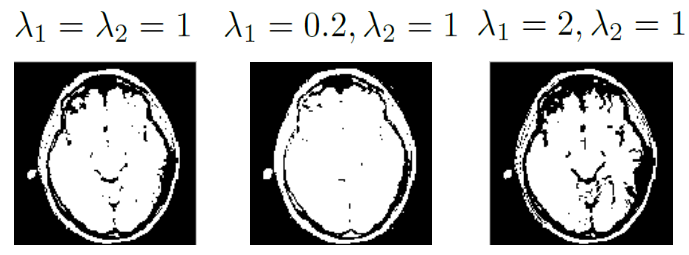
\includegraphics[width=0.5\textwidth]{cv_eg12.png}
\caption{Effect of varying $\lambda_1$ which controls how much details are detected inside the contour. The figure shows the final segmentation in each case.}
\label{fig:cv_eg12}
\end{figure*}

\begin{figure}[t!]
\centering
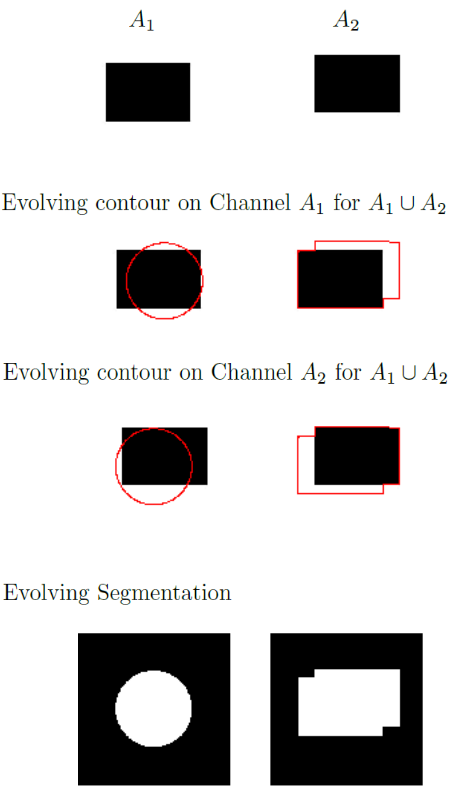
\includegraphics[width=6cm]{sc_unionsimple.png}
\caption{Simple union example. Size = 300 x 300, $\phi_{0}(x,y) = - \sqrt{(x - 150)^2 + (y - 150)^2} + 75$,  no reinitialization, cpu = 1.32 s, 
iterations = 2.}
\label{fig:sc_unionsimple}
\end{figure}

\begin{figure}[t!]
\centering
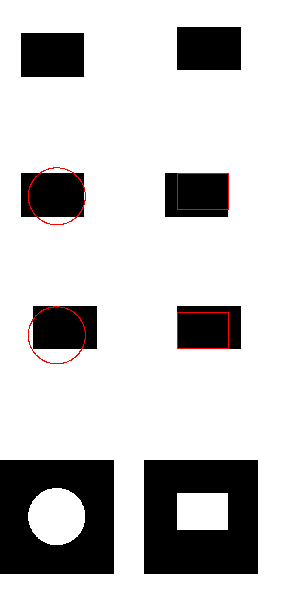
\includegraphics[width=6cm]{sc_intersectionsimple.png}
\caption{Simple intersection example. Size = 300 x 300, $\phi_{0}(x,y) = - \sqrt{(x - 150)^2 + (y - 150)^2} + 75$,  no reinitialization, cpu = 1.83 s, 
iterations = 2.}
\label{fig:sc_intersectionsimple}
\end{figure}


\subsubsection*{Logic Operators: union and intersection}

To ensure that the union operator is working properly, we tried it on a very simple example of two rectangles shown in Figure~\ref{fig:sc_unionsimple}. The
union of the two rectangles was successfully detected. Similarly, Figure~\ref{fig:sc_intersectionsimple} shows the intersection for the same two simple
rectangles. 

A practical usage of this logic operations framework is to recover missing parts from different images, and combine them to produce a more complete image. We
show this in Figure~\ref{fig:family} which shows two different version of a family image with a child missing in each image. When the union is applied to these
two channels, the complete family image is recovered.


Figure~\ref{fig:donutlogic} shows a more complicated example for both the intersection and union with the donut image shown in the previous section. We used
two versions of the donut with each one having a different part occluded. The results of the union and intersection operators are shown in the figure.
Additionally, this example shows that the Sandberg-Chan model can still successfully detect holes despite the addition of the logic operations.

We also wanted to make sure that the way the intensities in each channel are defined does not
matter. Figure~\ref{fig:diffint} shows the union and intersection performed on two channels of opposite intensities inside and outside the objects. The
segmentation was indeed contrast invariant as claimed by the authors. Finally, we show that our implementation can be extended to more than two channels.
Figure~\ref{fig:threech} shows the union, intersection, and the intersection of the union of three different channels.


\subsubsection*{Independence of Initial Curve Position}

\begin{figure*}[t!]
\centering
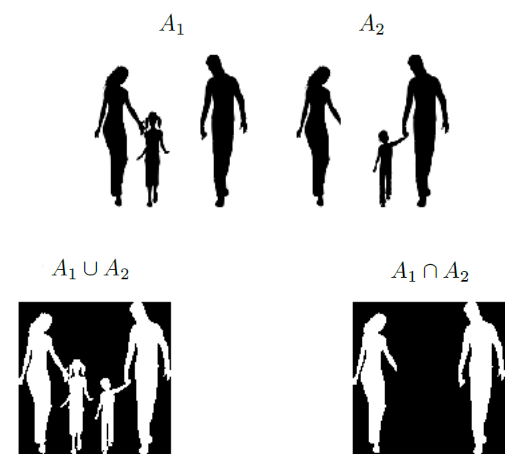
\includegraphics[width=0.3\textwidth]{family.png}
\caption{Combining missing information from two different channels. Size = 114 x 114. $\phi_{0}(x,y) = \sqrt{(x - 57)^2 + (y - 57)^2} -
28.5$, no reinitialization. Union: cpu = 4.01 s and iterations = 7. Intersection: cpu = 4.12 s and iterations = 7.}
\label{fig:family}
\end{figure*}

\begin{figure*}[t!]
\centering
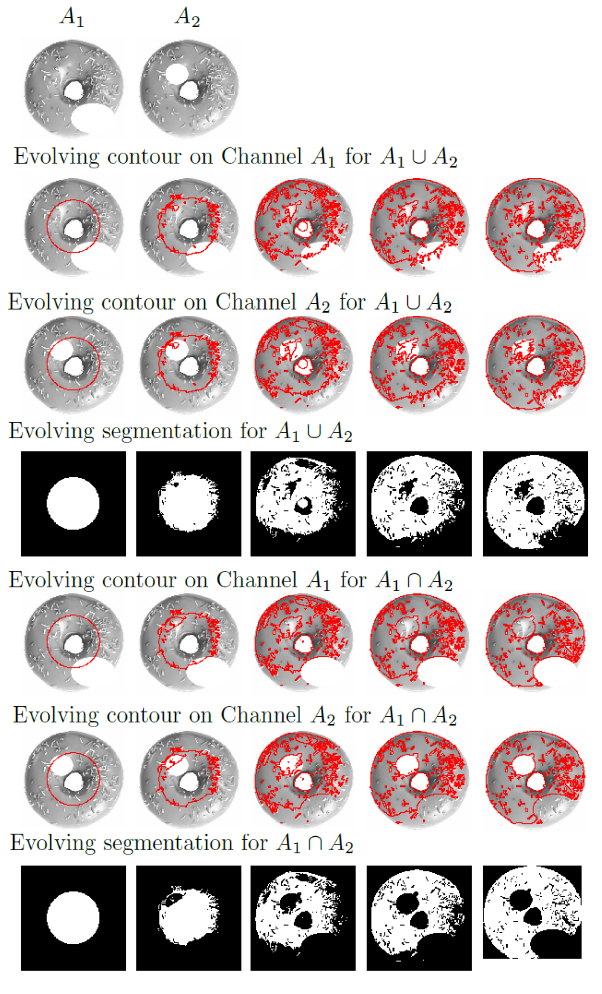
\includegraphics[width=0.5\textwidth]{donutlogic.png}
\caption{Performing union and intersection on images with holes. Size = 300 x 300. $\phi_{0}(x,y) = - \sqrt{(x - 150)^2 + (y - 150)^2)} +
75$, no reinitialization. For union: cpu = 8.63 sec and iterations = 10. For intersection: cpu = 7.68 sec and iterations = 10.}
\label{fig:donutlogic}
\end{figure*}

\begin{figure}[h!]
\centering
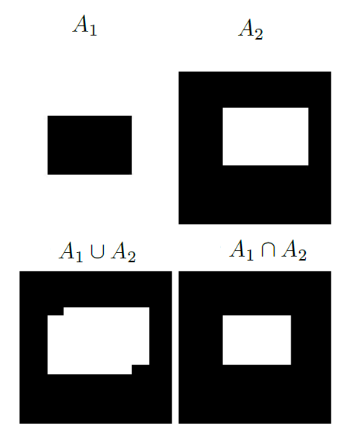
\includegraphics[width=0.3\textwidth]{diffint.png}
\caption{Segmentation for union and intersection of channels having reverse contrast.. Size = 300 x 300, $\phi_{0}(x,y) = - \sqrt{(x - 150)^2 + (y - 150)^2)} +
75$,  no reinitialization. For union: cpu = 1.32 sec and iterations = 2. For intersection: cpu = 1.83 sec and iterations = 2}
\label{fig:diffint}
\end{figure}

Similar to the previous model, we need to ensure that the position of the initial curve does not alter our results. Figure~\ref{fig:sc_position} shows
the segmentation results obtained for the same image used in Figure~\ref{fig:sc_unionsimple}, but with a different position for the initial curve. Both
segmentation are the same.


\subsubsection*{Reasonable Performance with Blurred Images}

Figure~\ref{fig:sc_blurry} shows the union performed on two blurry triangles. We blurred the triangles used in Figure~\ref{fig:threech}, and performed the
union operation on them. The full triangle was segmented (the union) despite the blurred edges.


\subsubsection*{Reasonable Performance with Noisy Images}

To be able to perform well in noisy images, $\lambda$ must be decreased in order to ignore the noise. We added \textit{Salt \& pepper} noise with a variation of
0.1 to
the images shown in Figure~\ref{fig:sc_noisy}, and tried to perform the union. In the first case shown, we set $\lambda = 255*255$ (i.e $ max(u)^2$) which is
the default setting
used for clean images, and in the second case, we set $\lambda = 125$. We show the final segmentation for both cases. In the first case, the noise was detected,
while in the second case, the noise was ignored since $\lambda$ was small. This shows that we also satisfy the response to parameter settings criteria since
$\lambda$ was the only variation mentioned by the authors in the original paper~\cite{sandberg2005logic}. We note that the contour evolved much more slowly
with a smaller $\lambda$, and thus took much more CPU time, and a larger number of iterations.

\begin{figure}[t!]
\centering
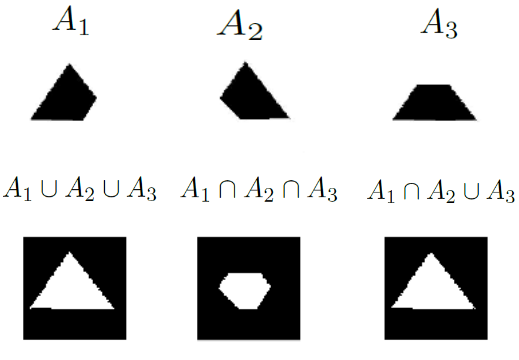
\includegraphics[width=0.3\textwidth]{threech.png}
\caption{Logic operations performed on three channels. The figure shows the final segmentation in each case. Size = 200 x 200. $\phi_{0}(x,y) = - \sqrt{(x -
100)^2 + (y - 100)^2} + 50$, $\mu = 0.1$, no reinitialization. For union: cpu = 3.92 sec and iterations = 6. For intersection: cpu = 3.11 sec and iterations =
5. For intersection then union: cpu = 1.24 and iterations = 4.}
\label{fig:threech}
\end{figure}

\begin{figure}[t]
\centering
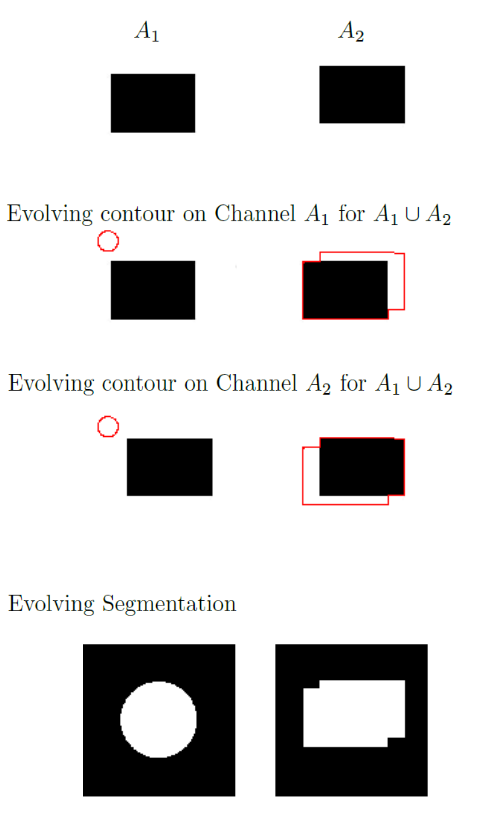
\includegraphics[width=0.3\textwidth]{sc_position.png}
\caption{Same example shown in Figure~\ref{fig:sc_unionsimple}, but with different initial curve position. Initial curve does not overlap with either objects.
Same segmentation is obtained. Size = 300 x 300, $\phi_{0}(x,y) = - \sqrt{(x - 150)^2 + (y - 150)^2)} + 75$,  no reinitialization, cpu = 4.43s, 4
iterations.}
\label{fig:sc_position}
\end{figure}



\subsubsection*{Complement}

Unfortunately, the complement did not work properly in our implementation. We closely followed the definitions in the original paper where $z_i^{in'} = 1 -
z_i^{in}$ and $z_i^{out'} = 1 - z_i^{out}$. The result was actually successfully detected, but continuous flickering occurred, and the curve did not stop
evolving We discuss this results in more details in Section~\ref{sec:difficulties}.

\subsubsection*{Other Tests}

Since the Sandberg-Chan model can successfully detect objects in one channel which are not in another when performing the union, we were curious to know
whether this would allow us to perform successful segmentation on colored images by combining the information in the three channels R,G,B. Accordingly, we used
the image in Figure~\ref{fig:cv_eg7} which the Chan-Vese model was not able to completely segment. We extracted three channels from the colored image: Red,
Green, Blue, and performed the union on the three channels. The results are shown in Figure~\ref{fig:flowers}. The complete contour of the flowers was
successfully detected unlike that obtained in Figure~\ref{fig:cv_eg7}.

\begin{figure*}[t]
\centering
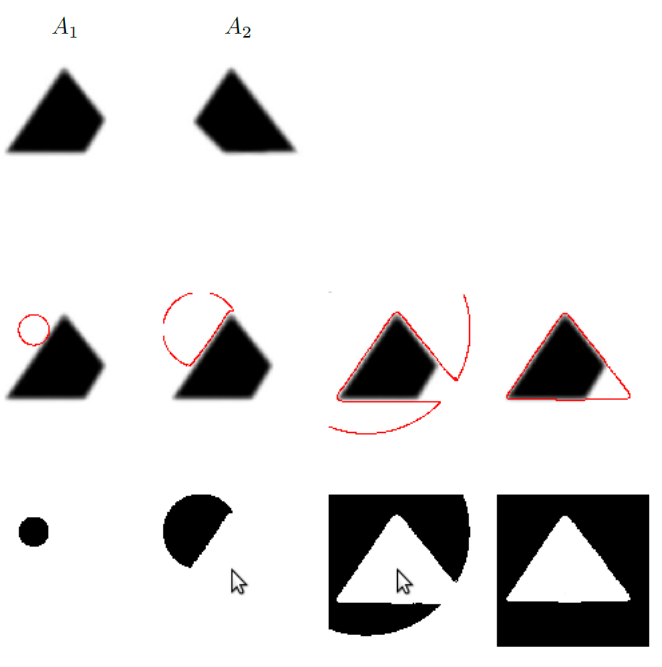
\includegraphics[width=0.3\textwidth]{sc_blurry.png}
\caption{Successful union with blurred images. Top: the evolving curve for $A_1 \cup A_2$
(in red) over time where the first
image shows the initial
contour. Bottom: evolving segmentation over time until the union is detected. Size = 200 x 200, $\phi_{0}(x,y) = - \sqrt{(x - 100)^2 + (y - 100)^2)} +
50$, no reinitialization, cpu = 6 s, iterations = 11.}
\label{fig:sc_blurry}
\end{figure*}

\begin{figure*}[t!h!]
\centering
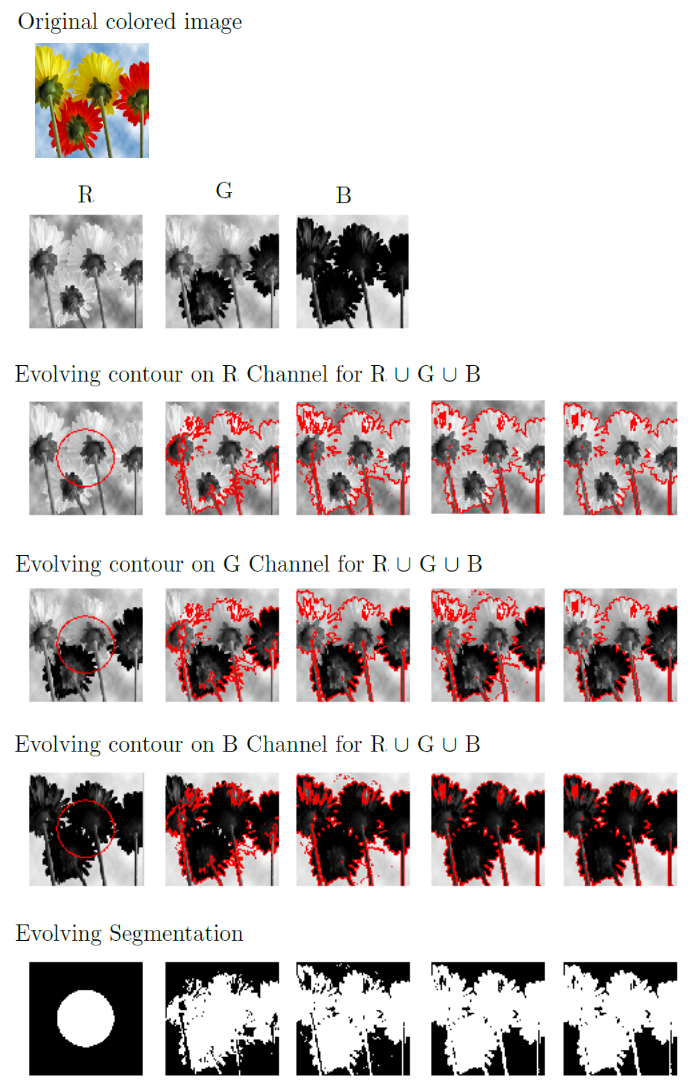
\includegraphics[width=0.5\textwidth]{flowers.png}
\caption{Ability to detect the full contour on a colored image with low variation between foreground and background by taking the union of the RGB channels.
Full contour detected as opposed to Figure~\ref{fig:cv_eg7}. Size = 300 x 300, $\phi_{0}(x,y) = - \sqrt{(x - 150)^2 + (y - 150)^2)} + 75$, no reinitialization,
size = cpu = 1.73 sec, iterations = 7.}
\label{fig:flowers}
\end{figure*}



\section{Difficulties and Discussion}
\label{sec:difficulties}
We have faced many challenges throughout the implementation of this project. Some of the challenges caused major delays in the implementation cycle and hindered
us from improving our code and adding more features to it. 

\subsection{Varying $\mu$}
$\mu$ is a scaling factor that is used in both the Chan-Vese model and the Sandberg-Chan model to control the weight given to the length of the contour.
Therefore, varying the value of $\mu$ will affect the ability to segment objects in noisy images, especially when the noise is similar to Matlab's \textit{salt
and pepper} noise. However, varying $\mu$ in our implementation does not really have any impact on the length of the contour. Figure~\ref{fig:cvmu} shows the
segmentation of an object in a noisy image for different values for $\mu$. The resulting segmentation is the same for all values of $\mu$. It is worth noting
that
this challenge kept us busy for over two days, after which we decided we should move on to other parts of the project.



\begin{figure}[t]
\centering
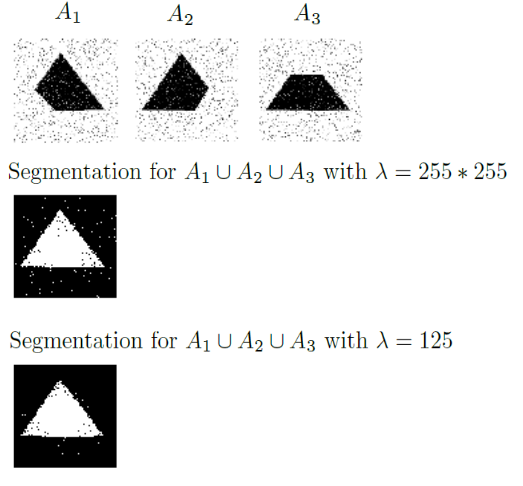
\includegraphics[width=0.4\textwidth]{sc_noisy.png}
\caption{Union of noisy channels. Same image as Figure~\ref{fig:threech}, but with \textit{Salt \& pepper'} noise with a variation of 0.1. Decreasing $\lambda$
from 255*255 to 125 allowed less
noise to be detected. Size = 200 x 200, $\phi_{0}(x,y) = - \sqrt{(x - 100)^2 + (y - 100)^2)} +
50$, no reinitialization. Cpu = 3.17 sec and iterations = 5 when $\lambda = 255*255$. Cpu = 146.46 sec and iterations = 125 when $\lambda =
125$.}
\label{fig:sc_noisy}
\end{figure}

\begin{figure}[t]
\centering
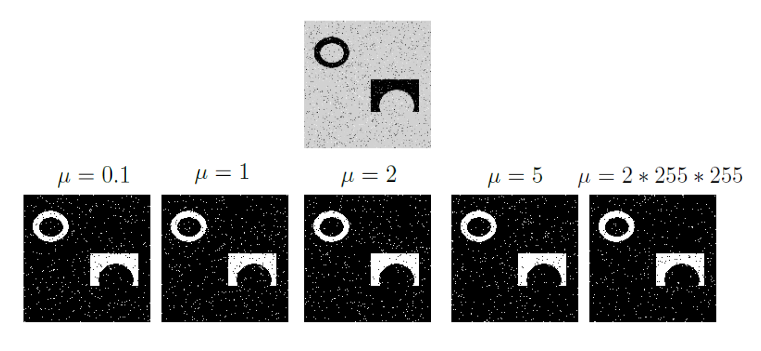
\includegraphics[width=0.5\textwidth]{cvmu.png}
\caption{$\mu$ does not have any effect on the length of the contour. \textit{Salt and pepper} noise was added to the original image for testing
purposes. Top: original image with noise. Bottom: segmentation for various values of $\mu$.}
\label{fig:cvmu}
\end{figure}

\subsection{Computing the Complement}
The Sandberg-Chan model supports the complement logic operator, so one can segment the logic object ($A \cap \neg B$) (i.e. segment what is in channel A and not
in channel B). The model defines the complement of the object in channel \textit{i} as follows:

\begin{equation}
\label{eqn:complement}
%\begin{align*}
{z_{i}}^{in^{'}} = 1 - {z_{i}}^{in}, \\
{z_{i}}^{out^{'}} = 1 - {z_{i}}^{out}.
%\end{align*}
\end{equation}

Although the definition is very simple, it did not work in practice. We implemented the complement logic operator as defined in Equation~\ref{eqn:complement},
and the segmentation does not stop at the required result. It rather keeps evolving after reaching the required solution, then keeps
flipping between two segmentations: the correct segmentation, and the segmentation of $A \cap B$. Figure~\ref{fig:sccomp} shows this scenario. We tried to
debug the reasons for this problem for three days.

\begin{figure}[t]
\centering
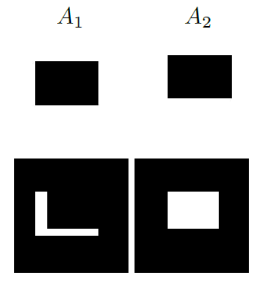
\includegraphics[width=0.25\textwidth]{sccomp.png}
\caption{The complement operator causes the contour to go through an infinite loop between two segmentations: the correct segmentation, and the segmentation
of $A_1 \cap A_2$. Bottom: correct and incorrect segmentation respectively}
\label{fig:sccomp}
\end{figure}

\subsection{Defining the initial contour $\phi_0$}
Both the Chan-Vese model and the Sandberg-Chan model define the initial contour ($\phi_0$) as a signed distance function where $\phi_0$ is positive inside the
contour $C$, zero on the boundary of $C$ ($\partial C$), and negative outside the contour $C$. Figure~\ref{fig:phinote} illustrates those assumptions.

\begin{figure}[t]
\centering
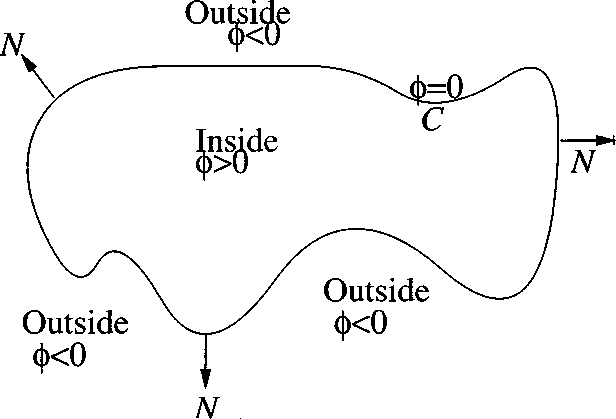
\includegraphics[width=0.3\textwidth]{phinote.png}
\caption{Assumptions about the way $\phi_0$ is defined.}
\label{fig:phinote}
\end{figure}

Since we model our initial contour as a circle, we have to modify the regular equation of the circle to match those assumption. Therefore, we initialize
$\phi_0$ as follows:

\begin{equation}
\label{eqn:phinote}
\phi_{0} (x, y) = radius - \sqrt{ (x - c_x)^2 + (y - c_y)^2 },
\end{equation}
where $c_x$ and $c_y$ are the x-coordinate and y-coordinate of the center of the circle respectively.

Although this definition of $\phi_0$ is compatible with most of the images we used to test our implementation, it did fail to correctly segment the objects in
some images. In fact, the results were the opposite of the used logic operator (i.e. the output is the intersection of the channels, while it should be the
union). After spending quite sometime to resolve this problem and checking what might be the source of the error, we tried using the regular equation of a
circle to initialize $\phi_0$ (Equation~\ref{eqn:phinotenormal}). We were very intrigued to notice that this modification resulted in the correct segmentation
of the input channels. Figure~\ref{fig:phidef} shows the final segmentation using both definitions for $\phi_0$.

\begin{equation}
\label{eqn:phinotenormal}
\phi_{0} (x, y) = \sqrt{ (x - c_x)^2 + (y - c_y)^2 } - radius,
\end{equation}
where $c_x$ and $c_y$ are the x-coordinate and y-coordinate of the center of the circle respectively.

\begin{figure}[t]
\centering
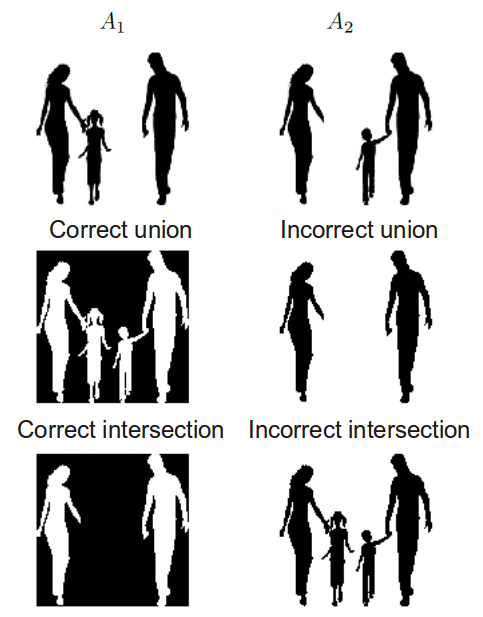
\includegraphics[width=0.4\textwidth]{phidef.png}
\caption{Union and intersection depending on the way $\phi$ is defined}
\label{fig:phidef}
\end{figure}

\subsection{Mistyped Equations}
As previously mentioned in Section~\ref{sec:sandberg-chan}, there is a typo in the equations that define $z_{in}$ and $z_{out}$ in the Sandberg-Chan model
(equation 3 in their paper). In addition, they have another typo in the expansion of the the Eular-Lagrange equation for the PDE that models the problem. Both
typos consumed over a week of our time until we were able to find out what are the correct equations in both cases. We could have spent this time overcoming
other challenges that we faced while implementing both models.

\section{Conclusion}
\label{sec:concl}
In this project, we have provided an implementation for the Chan-Vese model for active contours without edges and the Sandberg-Chan logic framework for
multi-channel images, both written in Matlab. Our experiments have shown that the Chan-Vese model is effective for various types of images. In specific, it is
useful when an edge-based segmentation is not applicable (i.e. edges do not depend on a gradient). However, our implementation fails to respond to different
values for the contour length scaling parameter, $\mu$. This affects the ability of our implementation to handle Matlab's \textit{Salt \& pepper} noise. On the
other hand, changing the values for the intensity weight parameters $\lambda_1$ and $\lambda_2$ affects the amount of details obtained inside and outside the
segmented object respectively.

We have also shown that our implementation for the Sandberg-Chan logic framework handles different logic combinations for multiple channels. We have also
experimented using it as a segmentation tool for colored images by modeling an input colored images as a 3-channels (red, green, blue). However, our
implementation for the \textit{complement} logic operation seems to be missing a hidden trick in the Sandberg-Chan logic framework.



\bibliography{references}
\bibliographystyle{ieee}

\appendix
\appendixpage

\section{Division of Labor}

We both implemented the Chan-Vese model together since this was the starting point of the project. Sarah did most of the initial implementation for the
Sandberg-Chan model by defining all the necessary functionalities for the logic operations for two images. Karim then extended it to multiple images. Karim
also tested the Sandberg-Chan model, and took most of the snapshots in that part for the paper. Sarah tested the Chan-Vese model, and took all its snapshots
for the paper. We both worked on finding an appropriate stopping condition for the contour evolution, and invested a lot of time to debug the problems we
faced that were described in Section~\ref{sec:difficulties}.



% insert where needed to balance the two columns on the last page with
% biographies
%\newpage

\end{document}



